\chapter{Euclidean Correlation Functions and Gaussian Perturbation Theory}
\label{ch:euclidean-correlation-functions-gaussian-perturbation}
\ConventionsEuclidean


\section{Spectral Correlators and Euclidean Time}

Let \(\widehat H\) be a self-adjoint Hamiltonian on a Hilbert space
\(\Hilb\). Assume in this section that \(\widehat H\) has a normalized
ground state \(\ket 0\) with energy \(E_0\), and that the example under
discussion admits a complete orthonormal basis \(\{\ket n\}\) of energy
eigenvectors,
\[
  \widehat H\ket n=E_n\ket n,\qquad E_n\ge E_0.
\]
For a self-adjoint coordinate operator \(\widehat q\), define the real-time
Heisenberg operator
\[
  \widehat q(t)
  =
  \exp\left(\frac{\ii}{\hbar}t\widehat H\right)
  \widehat q
  \exp\left(-\frac{\ii}{\hbar}t\widehat H\right),
  \qquad t\in\mathbb R.
\]
The ordered two-point function with the later insertion on the left is
\[
  W(t)=\bra 0\widehat q(t)\widehat q(0)\ket 0 .
\]
Inserting the energy basis gives
\[
\begin{aligned}
  W(t)
  &=
  \sum_n
  \bra 0\widehat q(0)\ket n
  \bra n\widehat q(0)\ket 0\,
  \exp\left[-\frac{\ii}{\hbar}(E_n-E_0)t\right]  \\
  &=
  \sum_n
  \left|\bra n\widehat q(0)\ket 0\right|^2
  \exp\left[-\frac{\ii}{\hbar}(E_n-E_0)t\right].
\end{aligned}
\]
The displayed sum is the pure-point case of a spectral-measure statement.
Let \(P_{\widehat H}\) be the projection-valued spectral measure of
\(\widehat H\), set
\[
\eta_q:=\widehat q\ket0,
\]
and define the positive Borel measure
\[
  \mu_q(B)=\langle \eta_q,P_{\widehat H}(B)\eta_q\rangle
\]
for Borel sets \(B\subset\mathbb R\).  Then, whenever
\(\eta_q\in\Hilb\), \(\mu_q\) is finite, has support in \([E_0,\infty)\),
and the two-point function is
\[
  W(t)=
  \int_{[E_0,\infty)}
  \exp\left[-\frac{\ii}{\hbar}(E-E_0)t\right]\,\dd\mu_q(E).
\]
For \(t=x+\ii y\) with \(y<0\), the integrand has modulus
\(\exp[(E-E_0)y/\hbar]\le1\).  Dominated convergence therefore gives a
holomorphic continuation of \(W(t)\) to the lower half \(t\)-plane.  The
discrete expansion above is recovered when \(\mu_q\) is a sum of atoms at
the eigenvalues \(E_n\).
For \(\tau>0\), define
\[
  G_E(\tau)
  =
  W(-\ii\tau)
  =
  \int_{[E_0,\infty)}
  \exp\left[-\frac{1}{\hbar}(E-E_0)\tau\right]\,\dd\mu_q(E),
\]
which in the pure-point case is
\[
  G_E(\tau)
  =
  \sum_n
  \left|\bra n\widehat q(0)\ket 0\right|^2
  \exp\left[-\frac{1}{\hbar}(E_n-E_0)\tau\right].
\]
Thus Euclidean time converts the spectral decomposition into a sum of
decaying exponentials. The decay rates are
\[
  \omega_n=\frac{E_n-E_0}{\hbar}.
\]

For \(\tau_1,\ldots,\tau_r\in\mathbb R\), let \(T_E\) denote Euclidean
ordering: operators with larger \(\tau\) are placed to the left. The Euclidean
\(r\)-point function of a single coordinate operator is
\[
  G_E^{(r)}(\tau_1,\ldots,\tau_r)
  =
  \bra 0
  T_E\{\widehat q_E(\tau_1)\cdots\widehat q_E(\tau_r)\}
  \ket 0,
\]
where
\[
  \widehat q_E(\tau)
  =
  \exp\left(\frac{1}{\hbar}\tau\widehat H\right)
  \widehat q
  \exp\left(-\frac{1}{\hbar}\tau\widehat H\right)
\]
is the analytic continuation of \(\widehat q(t)\) to \(t=-\ii\tau\).

It is useful to package the ordered functions by a source. For a smooth
compactly supported function \(J(\tau)\), define
\[
  Z_E[J]
  =
  \bra 0
  T_E
  \exp\left[
    \frac{1}{\hbar}
    \int_{\mathbb R}J(\tau)\widehat q_E(\tau)\,\dd\tau
  \right]
  \ket 0 .
\]
The correlation functions are obtained by
\[
  G_E^{(r)}(\tau_1,\ldots,\tau_r)
  =
  \left.
  \hbar^r
  \frac{\delta}{\delta J(\tau_1)}
  \cdots
  \frac{\delta}{\delta J(\tau_r)}
  Z_E[J]
  \right|_{J=0}.
\]

\section{Wick Rotation of the Path Integral}

Consider a Lagrangian of the form
\[
  L(q,\dot q)
  =
  \frac12G_{ab}(q)\dot q^a\dot q^b-V(q),
\]
where \(G_{ab}(q)\) is positive definite. Under the analytic continuation
\[
  t=-\ii\tau,\qquad
  \dot q^a=\frac{\dd q^a}{\dd t}
  =
  \ii\,\frac{\dd q^a}{\dd\tau},
\]
define the Euclidean Lagrangian
\[
  L_E(q,q')
  =
  -L(q,\ii q'),
  \qquad q'^a=\frac{\dd q^a}{\dd\tau}.
\]
For the displayed \(L\), this gives
\[
  L_E(q,q')
  =
  \frac12G_{ab}(q)q'^aq'^b+V(q).
\]
The Lorentzian phase transforms as
\[
  \exp\left[
    \frac{\ii}{\hbar}\int L(q,\dot q)\,\dd t
  \right]
  \longmapsto
  \exp\left[
    -\frac{1}{\hbar}\int L_E(q,q')\,\dd\tau
  \right].
\]

Let \(\ket\psi\in\Hilb\) satisfy \(\braket{0}{\psi}\ne0\), and assume for this
paragraph that the ground state is separated from the rest of the spectrum by
a gap.  Write
\[
  \ket\psi=c_0\ket0+\ket{\psi_\perp},
  \qquad c_0=\braket{0}{\psi},
  \qquad \braket{0}{\psi_\perp}=0,
\]
and let the spectrum of \(\widehat H-E_0\) on the closed subspace
\[
  \{\ket0\}^\perp
  =
  \{\eta\in\Hilb:\braket{0}{\eta}=0\}
\]
lie in \([\Delta,\infty)\) with \(\Delta>0\).  Spectral calculus gives
\[
  \ee^{-T(\widehat H-E_0)/\hbar}\ket\psi
  =
  c_0\ket0+O(\ee^{-T\Delta/\hbar})
\]
in Hilbert norm.  Therefore
\[
  \frac{\exp[-T(\widehat H-E_0)/\hbar]\ket\psi}
       {\left\|\exp[-T(\widehat H-E_0)/\hbar]\ket\psi\right\|}
  \longrightarrow
  \frac{c_0}{|c_0|}\ket0
\]
as \(T\to\infty\).  The phase \(c_0/|c_0|\) cancels between bra and ket in
vacuum expectation values.  For \(0<\tau_1<\cdots<\tau_r<T\), the
Euclidean correlation function is the long-time limit of matrix elements of
\(\exp(-\tau\widehat H/\hbar)\) with insertions at the specified Euclidean
times.

The same limit may be represented before Wick rotation by a regulated path
integral on a complex-time contour.  Let \(\Gamma_{T,t}\) run from
\(t_i=\ii T\) to \(0\), then along the real segment from \(0\) to \(t\),
and then to \(t_f=t-\ii T\), so that
\[
  \operatorname{Im} t_i\to+\infty,
  \qquad
  \operatorname{Im} t_f\to-\infty
\]
as \(T\to\infty\).  If \([Dq]_{\Gamma,\psi}\) denotes the time-sliced
measure on this contour with endpoint wavefunctions of a vector \(\ket\psi\)
included, then
\[
  \bra 0\widehat q(t)\widehat q(0)\ket 0
  =
  \lim_{T\to\infty}
  \frac{
    \int [Dq]_{\Gamma_{T,t},\psi}\,
    \exp\left[
      \frac{\ii}{\hbar}\int_{\Gamma_{T,t}}
      L(q,\dot q)\,\dd t
    \right]q(t)q(0)
  }{
    \int [Dq]_{\Gamma_{T,t},\psi}\,
    \exp\left[
      \frac{\ii}{\hbar}\int_{\Gamma_{T,t}}
      L(q,\dot q)\,\dd t
    \right]
  },
\]
under the same ground-state overlap and gap hypotheses.  This formula is a
contour version of the operator projection above; the regulator and endpoint
data are part of \([Dq]_{\Gamma,\psi}\).

\begin{center}
\begin{tikzpicture}[>=Stealth,scale=0.95]
  \draw[->] (-0.65,0) -- (3.5,0) node[right] {$\operatorname{Re}t$};
  \draw[->] (0,-2.05) -- (0,2.15) node[above] {$-\operatorname{Im}t$};
  \draw[blue!70!black,line width=1.05pt,->] (0,-1.72) -- (0,-0.08);
  \draw[green!45!black,line width=1.05pt,->] (0,0) -- (2.15,0);
  \draw[purple!75!black,line width=1.05pt,->] (2.15,0.05) -- (2.15,1.75);
  \fill[orange] (0,0) circle (2pt) node[below left=2pt] {$0$};
  \fill[red] (2.15,0) circle (2pt) node[below=2pt] {$t$};
  \node[blue!70!black,left] at (0,-1.6) {$t_i$};
  \node[purple!75!black,right] at (2.15,1.6) {$t_f$};
  \node[green!45!black,above] at (1.15,0.05) {real segment};
\end{tikzpicture}
\end{center}

After the Wick rotation of the contour to Euclidean time, the Lagrangian
path-integral notation becomes
\[
  \bra 0T_E\{\widehat q_E(\tau_1)\cdots\widehat q_E(\tau_r)\}\ket 0
  =
  \lim_{T\to\infty}
  \frac{
    \int [Dq]\,\exp[-S_E[q]/\hbar]\,
    q(\tau_1)\cdots q(\tau_r)
  }{
    \int [Dq]\,\exp[-S_E[q]/\hbar]
  },
\]
where the symbol \([Dq]\) denotes a specified regulator and limiting
procedure, and
\[
  S_E[q]=\int_{-T}^{T}L_E(q,q')\,\dd\tau.
\]

\begin{center}
\begin{tikzpicture}[>=Stealth,scale=0.95]
  \draw[->] (-3.2,0) -- (3.35,0) node[right] {$\operatorname{Re}t$};
  \draw[->] (0,-2.15) -- (0,2.15) node[above] {$-\operatorname{Im}t=\tau$};
  \draw[blue!70!black,line width=1pt,->] (0,0) -- (2.05,0);
  \node[blue!70!black,below] at (1.1,0) {real time};
  \draw[green!45!black,line width=1pt,->] (0,0) -- (0,1.75);
  \node[green!45!black,anchor=west] at (0.18,1.55) {Euclidean time};
  \draw[orange!80!black,line width=0.9pt,->]
    (1.45,0) arc[start angle=0,end angle=90,radius=1.45];
  \node[orange!80!black] at (1.28,0.82) {$t=-\ii\tau$};
  \fill (0,0) circle (1.8pt);
\end{tikzpicture}
\end{center}

\begin{center}
\begin{tikzpicture}[>=Stealth,scale=0.95]
  \draw[->] (-3.2,0) -- (3.35,0) node[right] {$\tau$};
  \draw[line width=0.8pt,blue!65!black] (-2.6,0) -- (2.6,0);
  \foreach \x/\lab in {-2.6/{-T},0/{0},1.15/{\tau},2.6/{T}} {
    \fill (\x,0) circle (2pt);
    \node[below=3pt] at (\x,0) {$\lab$};
  }
  \draw[decorate,decoration={brace,amplitude=4pt}]
    (-2.6,0.35) -- node[midway,above=5pt] {\scriptsize projection} (0,0.35);
  \draw[decorate,decoration={brace,amplitude=4pt,mirror}]
    (0,-0.42) -- node[midway,below=5pt] {\scriptsize ordered insertions} (1.15,-0.42);
  \draw[decorate,decoration={brace,amplitude=4pt}]
    (1.15,0.35) -- node[midway,above=5pt] {\scriptsize projection} (2.6,0.35);
\end{tikzpicture}
\end{center}

A concrete evaluation begins by specifying the regulator.  One common
choice is a mode cutoff: choose functions \(f_n(\tau)\), write
\[
  q(\tau)=\sum_{n=1}^{N_{\rm max}}q_nf_n(\tau),
\]
and define the regulated measure by a finite product of Lebesgue measures in
the coefficients \(q_n\), together with whatever normalization and boundary
conditions are dictated by the time-sliced construction.  The limit
\(N_{\rm max}\to\infty\) is then a further analytic step.  The harmonic
oscillator provides the basic Gaussian example.

\section{The Harmonic Oscillator}

Let
\[
  \widehat H=\frac12(\widehat p^2+\omega^2\widehat q^2),
  \qquad
  L(q,\dot q)=\frac12\dot q^2-\frac12\omega^2q^2,
\]
with \(\omega>0\). The Euclidean action on the interval \([-T,T]\) is
\[
  S_E[q]
  =
  \frac12\int_{-T}^{T}
  \left[
    (q')^2+\omega^2q^2
  \right]\dd\tau .
\]
Impose Dirichlet boundary conditions \(q(-T)=q(T)=0\) and expand
\[
  q(\tau)=\sum_{n=1}^{\infty}q_nf_n(\tau),
  \qquad
  f_n(\tau)=\frac{1}{\sqrt T}
  \sin\frac{n\pi(\tau+T)}{2T}.
\]
The functions \(f_n\) obey
\[
  \int_{-T}^{T}f_n(\tau)f_m(\tau)\,\dd\tau=\delta_{nm},
  \qquad
  -\frac{\dd^2}{\dd\tau^2}f_n
  =
  \left(\frac{n\pi}{2T}\right)^2f_n .
\]
Consequently
\[
  S_E[q]
  =
  \frac12\sum_{n=1}^{\infty}
  \left[
    \left(\frac{n\pi}{2T}\right)^2+\omega^2
  \right]q_n^2 .
\]

\begin{center}
\begin{tikzpicture}[>=Stealth,scale=0.95]
  \draw[->] (-3.2,0) -- (3.4,0) node[right] {$\tau$};
  \draw[->] (0,-1.15) -- (0,1.55) node[above] {$q(\tau)$};
  \draw[purple!80!black,line width=1pt]
    (-2.55,0)
    .. controls (-2.05,0.75) and (-1.38,0.95) .. (-0.92,0.05)
    .. controls (-0.52,-0.82) and (-0.12,-0.74) .. (0.25,0.22)
    .. controls (0.74,1.18) and (1.65,0.98) .. (2.55,0);
  \fill (-2.55,0) circle (2pt) node[below] {$-T$};
  \fill (2.55,0) circle (2pt) node[below] {$T$};
  \node[below] at (0,-1.0) {$q(-T)=q(T)=0$};
\end{tikzpicture}
\end{center}

Define the normalized finite-\(T\) expectation value by
\[
  \langle F\rangle_T
  =
  \frac{
    \int\prod_{n=1}^{\infty}\dd q_n\,
    \exp[-S_E[q]/\hbar]\,F
  }{
    \int\prod_{n=1}^{\infty}\dd q_n\,
    \exp[-S_E[q]/\hbar]
  },
\]
with the understanding that a finite mode cutoff is used before the limiting
operation. The independent Gaussian integrals give
\[
  \langle q_nq_m\rangle_T
  =
  \delta_{nm}\,
  \frac{\hbar}{
    \left(\frac{n\pi}{2T}\right)^2+\omega^2
  }.
\]
Therefore
\[
  \langle q(\tau_1)q(\tau_2)\rangle_T
  =
  \sum_{n=1}^{\infty}
  \frac{\hbar\,f_n(\tau_1)f_n(\tau_2)}
       {\left(\frac{n\pi}{2T}\right)^2+\omega^2}.
\]
The passage to the infinite Euclidean line is not a formal replacement of a
sum by an integral; it is a limit at fixed insertion points.  Set
\[
  k_n=\frac{n\pi}{2T},
  \qquad
  \Delta k=\frac{\pi}{2T}.
\]
Using the explicit sine basis,
\[
\begin{aligned}
  \langle q(\tau_1)q(\tau_2)\rangle_T
  &=
  \sum_{n=1}^{\infty}
  \frac{\hbar}{T}
  \frac{
    \sin k_n(\tau_1+T)\sin k_n(\tau_2+T)
  }{k_n^2+\omega^2}  \\
  &=
  \frac{2\hbar}{\pi}
  \sum_{n=1}^{\infty}\Delta k\,
  \frac{
    \sin k_n(\tau_1+T)\sin k_n(\tau_2+T)
  }{k_n^2+\omega^2}.
\end{aligned}
\]
To state the limit as an operation on the regulated path integral, insert
temporarily an Abel factor \(\ee^{-\varepsilon k_n}\), \(\varepsilon>0\), in
the mode sum and the corresponding factor \(\ee^{-\varepsilon k}\) in the
continuum integral.  The Riemann limit is then taken at fixed
\(\varepsilon\), and the limit \(\varepsilon\downarrow0\) is taken after the
Fourier integral has been evaluated.  Suppressing this auxiliary factor from
the notation, the continuum expression is
\[
  \frac{2\hbar}{\pi}
  \int_{0}^{\infty}\dd k\,
  \frac{
    \sin k(\tau_1+T)\sin k(\tau_2+T)
  }{k^2+\omega^2}.
\]
Writing \(2\sin a\sin b=\cos(a-b)-\cos(a+b)\), equivalently
\[
\begin{aligned}
  \langle q(\tau_1)q(\tau_2)\rangle_T
  &=
  \frac{\hbar}{\pi}
  \int_{-\infty}^{\infty}\frac{\dd k}{k^2+\omega^2}
  \biggl[
    \frac14\ee^{\ii k(\tau_1-\tau_2)}
    +\frac14\ee^{-\ii k(\tau_1-\tau_2)}  \\
  &\hspace{5.0cm}
    -\frac14\ee^{\ii k(\tau_1+\tau_2+2T)}
    -\frac14\ee^{-\ii k(\tau_1+\tau_2+2T)}
  \biggr]
  +o(1),
\end{aligned}
\]
where \(o(1)\) denotes the regulator error in the infinite-volume limit.
Thus the finite interval produces, besides the translation-invariant term, an
image term tied to the Dirichlet endpoints.

The elementary Fourier integral needed here is
\[
  I(\tau)
  =
  \int_{-\infty}^{\infty}
  \frac{\ee^{\ii k\tau}}{k^2+\omega^2}\,\dd k .
\]
For \(\tau>0\), \(|\ee^{\ii k\tau}|=\ee^{-(\operatorname{Im}k)\tau}\), so the
large semicircle is suppressed in the upper half-plane and the pole enclosed
is \(k=\ii\omega\).  Therefore
\[
  I(\tau)
  =
  \frac{\pi}{\omega}\ee^{-\omega\tau}.
\]
For \(\tau<0\), close the contour in the lower half-plane and obtain
\(\pi\omega^{-1}\ee^{\omega\tau}\).

\begin{center}
\begin{tikzpicture}[>=Stealth,scale=0.98]
  \draw[line width=0.6pt] (-2.65,-1.75) rectangle (2.65,1.75);
  \draw[->] (-2.35,0) -- (2.35,0) node[right] {$\operatorname{Re}k$};
  \draw[->] (0,-1.45) -- (0,1.45) node[above] {$\operatorname{Im}k$};
  \draw[green!45!black,line width=1pt,->]
    (-2.0,0) arc[start angle=180,end angle=25,radius=2.0];
  \draw[green!45!black,line width=1pt]
    (1.81,0.84) arc[start angle=25,end angle=0,radius=2.0];
  \node[red!80!black] at (0,0.95) {$\times$};
  \node[right=2pt] at (0,0.95) {$\ii\omega$};
  \node[red!80!black] at (0,-0.95) {$\times$};
  \node[right=2pt] at (0,-0.95) {$-\ii\omega$};
  \node[align=center] at (0,-1.95) {upper contour for \(\tau>0\)};
\end{tikzpicture}
\end{center}

For fixed \(\tau_1,\tau_2\), the quantity \(\tau_1+\tau_2+2T\) is positive for
large \(T\), and the preceding integral gives
\[
  \langle q(\tau_1)q(\tau_2)\rangle_T
  =
  \frac{\hbar}{2\omega}\ee^{-\omega|\tau_1-\tau_2|}
  -
  \frac{\hbar}{2\omega}\ee^{-\omega(\tau_1+\tau_2+2T)}
  +o(1).
\]
The second term is the endpoint image contribution and vanishes as
\(T\to\infty\).  Hence the Euclidean two-point function of the harmonic
oscillator on the line is
\[
  \boxed{
  \langle q(\tau_1)q(\tau_2)\rangle
  =
  \frac{\hbar}{2\omega}
  \ee^{-\omega|\tau_1-\tau_2|}
  }.
\]
This agrees with the spectral expression, since the first operator
\(\widehat q\) connects the ground state of the harmonic oscillator to the
first excited state.

\section{Gaussian Integrals and Wick Pairings}

For the remainder of the chapter set \(\hbar=1\), unless \(\hbar\) is
displayed explicitly. Let \(A\) be a real symmetric positive-definite \(N\times N\)
matrix, and let \(J\in\mathbb R^N\). Define
\[
  Z_A[J]
  =
  \int_{\mathbb R^N}\dd^Nq\,
  \exp\left(
    -\frac12q_iA_{ij}q_j+J_iq_i
  \right),
\]
where repeated finite indices are summed. Completing the square gives
\[
  Z_A[J]
  =
  (2\pi)^{N/2}(\det A)^{-1/2}
  \exp\left(
    \frac12J_i(A^{-1})_{ij}J_j
  \right).
\]
The normalized Gaussian expectation of a function \(F(q)\) is
\[
  \langle F(q)\rangle_A
  =
  \frac{1}{Z_A[0]}
  \int_{\mathbb R^N}\dd^Nq\,
  \exp\left(-\frac12q_iA_{ij}q_j\right)F(q).
\]
Differentiating with respect to \(J\) gives
\[
  \langle F(q)\rangle_A
  =
  \left.
  F\left(\frac{\partial}{\partial J}\right)
  \frac{Z_A[J]}{Z_A[0]}
  \right|_{J=0}.
\]
Let \(C=A^{-1}\).  Then
\[
  \langle q_i\rangle_A
  =
  \left.
  \frac{\partial}{\partial J_i}
  \exp\left(\frac12J_aC_{ab}J_b\right)
  \right|_{J=0}
  =
  0
\]
and
\[
  \langle q_iq_j\rangle_A
  =
  \left.
  \frac{\partial}{\partial J_i}
  \frac{\partial}{\partial J_j}
  \exp\left(\frac12J_aC_{ab}J_b\right)
  \right|_{J=0}
  =
  C_{ij}.
\]
Write \(\partial_i=\partial/\partial J_i\).  For four variables,
\[
\begin{aligned}
  \langle q_iq_jq_kq_\ell\rangle_A
  &=
  \left.
  \partial_i\partial_j\partial_k\partial_\ell
  \exp\left(\frac12J_aC_{ab}J_b\right)
  \right|_{J=0}  \\
  &=
  \left.
  \partial_i\partial_j\partial_k\partial_\ell
  \frac12\left(\frac12J_aC_{ab}J_b\right)^2
  \right|_{J=0}  \\
  &=
  C_{ij}C_{k\ell}+C_{ik}C_{j\ell}+C_{i\ell}C_{jk}.
\end{aligned}
\]
Only the quadratic term squared in the exponential can survive after four
source derivatives and then setting \(J=0\).  The four derivatives can be
assigned to the four source factors in \(4!\) ways; these assignments group
into the three displayed pairings, and the numerical factor
\(\frac12(\frac12)^2=\frac18\) cancels the repeated orientations and the
exchange of the two covariance factors inside each pairing.

\begin{center}
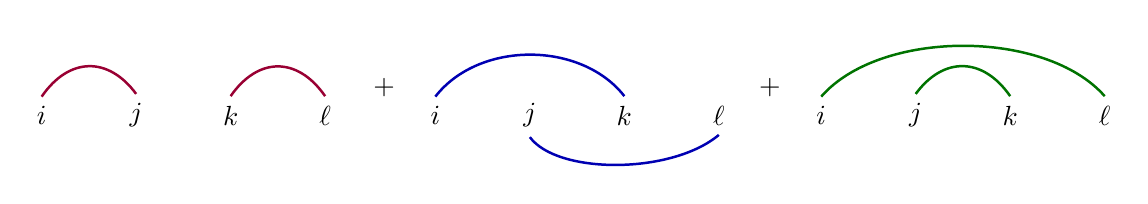
\begin{tikzpicture}[scale=1.0]
  \node (i) at (0,0) {$i$};
  \node (j) at (1.2,0) {$j$};
  \node (k) at (2.4,0) {$k$};
  \node (l) at (3.6,0) {$\ell$};
  \draw[purple!80!black,line width=0.9pt]
    (i.north) .. controls (0.35,0.75) and (0.85,0.75) .. (j.north);
  \draw[purple!80!black,line width=0.9pt]
    (k.north) .. controls (2.75,0.75) and (3.25,0.75) .. (l.north);
  \node at (4.35,0.35) {$+$};
  \node (i2) at (5.0,0) {$i$};
  \node (j2) at (6.2,0) {$j$};
  \node (k2) at (7.4,0) {$k$};
  \node (l2) at (8.6,0) {$\ell$};
  \draw[blue!70!black,line width=0.9pt]
    (i2.north) .. controls (5.55,0.95) and (6.85,0.95) .. (k2.north);
  \draw[blue!70!black,line width=0.9pt]
    (j2.south) .. controls (6.55,-0.75) and (8.0,-0.75) .. (l2.south);
  \node at (9.25,0.35) {$+$};
  \node (i3) at (9.9,0) {$i$};
  \node (j3) at (11.1,0) {$j$};
  \node (k3) at (12.3,0) {$k$};
  \node (l3) at (13.5,0) {$\ell$};
  \draw[green!45!black,line width=0.9pt]
    (i3.north) .. controls (10.65,1.1) and (12.75,1.1) .. (l3.north);
  \draw[green!45!black,line width=0.9pt]
    (j3.north) .. controls (11.45,0.75) and (11.95,0.75) .. (k3.north);
\end{tikzpicture}
\end{center}

A Wick contraction is an assigned pairing of two labels with value
\[
  (q_iq_j)_{\mathrm{contr}}=C_{ij}=(A^{-1})_{ij}.
\]
Wick's theorem says that the Gaussian expectation of \(2r\) variables is the
sum over all complete pairings, with one covariance factor for each pair:
\[
  \langle q_{i_1}\cdots q_{i_{2r}}\rangle_A
  =
  \sum_{\text{complete pairings }P}
  \prod_{(a,b)\in P}(A^{-1})_{i_ai_b}.
\]
Gaussian expectations of an odd number of variables vanish.

\section{Gaussian Functional Integrals}

Let \(A\) be the positive operator
\[
  A=-\frac{\dd^2}{\dd\tau^2}+\omega^2
\]
on a function space with boundary conditions for which \(A\) is invertible.
The Green function \(G(\tau,\tau')\) is the integral kernel of \(A^{-1}\):
\[
  (A^{-1}f)(\tau)
  =
  \int G(\tau,\tau')f(\tau')\,\dd\tau',
\]
and therefore satisfies
\[
  \left(
    -\frac{\dd^2}{\dd\tau^2}+\omega^2
  \right)G(\tau,\tau')
  =
  \delta(\tau-\tau').
\]
With the inner product
\[
  (f,g)=\int f(\tau)g(\tau)\,\dd\tau,
\]
the Gaussian Euclidean action is
\[
  S_0[q]=\frac12(q,Aq).
\]
The source-dependent Gaussian functional integral is defined by a regulator,
for instance a finite-mode cutoff, and has the finite-dimensional form in the
cutoff variables. Its continuum notation is
\[
  Z_0[J]
  =
  \int[Dq]\,
  \exp\left[
    -\frac12(q,Aq)+(J,q)
  \right].
\]
The ratio independent of normalization is
\[
  \frac{Z_0[J]}{Z_0[0]}
  =
  \exp\left[
    \frac12\int J(\tau)G(\tau,\tau')J(\tau')\,
    \dd\tau\,\dd\tau'
  \right].
\]
Consequently
\[
  \langle q(\tau_1)q(\tau_2)\rangle_0
  =
  G(\tau_1,\tau_2).
\]
The same result can be obtained without tracking the normalization of the
functional measure under discretization.  At finite cutoff this is ordinary
integration by parts in finitely many variables; the continuum notation is the
limit of that identity.  The functional derivative is normalized by
\[
  \frac{\delta q(\tau_2)}{\delta q(\tau')}=\delta(\tau'-\tau_2).
\]
Since
\[
  \frac{\delta}{\delta q(\tau')}
  \exp\left[-\frac12(q,Aq)\right]
  =
  -(Aq)(\tau')\exp\left[-\frac12(q,Aq)\right],
\]
one has
\[
  q(\tau_1)\exp\left[-\frac12(q,Aq)\right]
  =
  -
  \left(A^{-1}\frac{\delta}{\delta q}\right)(\tau_1)
  \exp\left[-\frac12(q,Aq)\right],
\]
where
\[
  \left(A^{-1}\frac{\delta}{\delta q}\right)(\tau_1)
  =
  \int G(\tau_1,\tau')\frac{\delta}{\delta q(\tau')}\,\dd\tau'.
\]
The regulated Gaussian has no boundary term in this finite-dimensional
integration by parts. Therefore
\[
\begin{aligned}
  &\int[Dq]\,\exp\left[-\frac12(q,Aq)\right]
    q(\tau_1)q(\tau_2)  \\
  &\quad =
  \int[Dq]\,\exp\left[-\frac12(q,Aq)\right]
  \left(A^{-1}\frac{\delta}{\delta q}\right)(\tau_1)q(\tau_2)  \\
  &\quad =
  \int[Dq]\,\exp\left[-\frac12(q,Aq)\right]
  \int G(\tau_1,\tau')\delta(\tau'-\tau_2)\,\dd\tau' .
\end{aligned}
\]
After division by \(Z_0[0]\), this gives again
\(\langle q(\tau_1)q(\tau_2)\rangle_0=G(\tau_1,\tau_2)\).

On the infinite Euclidean line, write
\[
  q(\tau)=
  \int_{-\infty}^{\infty}\frac{\dd k}{2\pi}\,
  \widetilde q(k)\ee^{\ii k\tau},
  \qquad
  \widetilde q(k)^*=\widetilde q(-k).
\]
Then
\[
  S_0[q]
  =
  \frac12
  \int_{-\infty}^{\infty}\frac{\dd k}{2\pi}\,
  \widetilde q(-k)(k^2+\omega^2)\widetilde q(k),
\]
and
\[
  \langle \widetilde q(k_1)\widetilde q(k_2)\rangle_0
  =
  \frac{2\pi\delta(k_1+k_2)}{k_1^2+\omega^2}.
\]
Thus
\[
  G(\tau,\tau')
  =
  \int_{-\infty}^{\infty}
  \frac{\dd k}{2\pi}\,
  \frac{\ee^{\ii k(\tau-\tau')}}{k^2+\omega^2}
  =
  \frac{1}{2\omega}\ee^{-\omega|\tau-\tau'|}.
\]

\section{The Anharmonic Oscillator}

Set \(\omega=1\) in this section. The anharmonic oscillator is defined by
\[
  \widehat H
  =
  \frac12\widehat p^2+\frac12\widehat q^2+\frac{g}{4!}\widehat q^4.
\]
For real \(g\ge0\), this differential operator on \(C_c^\infty(\mathbb R)\)
has a unique self-adjoint closure by the Faris--Lavine criterion stated in
Chapter~\ref{ch:hamiltonian-evolution-time-sliced-path-integrals}: the
potential
\[
  V(q)=\frac12q^2+\frac{g}{4!}q^4
\]
is smooth, bounded below, locally Kato, and has zero negative part.  Hence the
Euclidean semigroup and its time-sliced approximants are defined before the
perturbative expansion in \(g\) is formed.
The Euclidean Lagrangian is
\[
  L_E(q,q')
  =
  \frac12(q')^2+\frac12q^2+\frac{g}{4!}q^4.
\]
Let
\[
  S_0[q]=\int\left[\frac12(q')^2+\frac12q^2\right]\dd\tau,
  \qquad
  S_{\mathrm{int}}[q]=\frac{g}{4!}\int q(\tau)^4\,\dd\tau .
\]
At finite cutoff, perturbation theory is the coefficientwise expansion of
\(\exp[-S_{\mathrm{int}}]\) inside a finite-dimensional Gaussian integral:
\[
  \ee^{-S_{\mathrm{int}}[q]}
  =
  \sum_{n=0}^{\infty}
  \frac{1}{n!}
  \left(-\frac{g}{4!}\int q(\tau)^4\,\dd\tau\right)^n .
\]
No convergence of the infinite-dimensional integral or of the resulting power
series in \(g\) is assumed at this point; the coefficients are first defined in
the regulated Gaussian integral, and limits are then discussed coefficient by
coefficient.
For the partition function,
\[
  Z_g=\int[Dq]\,\exp[-S_0[q]-S_{\mathrm{int}}[q]],
\]
one obtains
\[
  \frac{Z_g}{Z_0}
  =
  \sum_{n=0}^{\infty}
  \frac{1}{n!}
  \left(-\frac{g}{4!}\right)^n
  \int \dd\tau_1\cdots\dd\tau_n\,
  \left\langle
    q(\tau_1)^4\cdots q(\tau_n)^4
  \right\rangle_0 .
\]
Here \(Z_0\) is the Gaussian partition function and
\(\langle\cdots\rangle_0\) is evaluated with
\[
  G_0(\tau,\tau')=\frac12\ee^{-|\tau-\tau'|}.
\]

At first order in \(g\),
\[
  -\frac{g}{4!}\int\dd\tau\,\langle q(\tau)^4\rangle_0
  =
  -\frac{g}{8}\int\dd\tau\,G_0(\tau,\tau)^2.
\]
The factor \(3\) in \(\langle q^4\rangle_0=3G_0(\tau,\tau)^2\) is the number
of pairings of four fields at the vertex.
Since \(G_0(\tau,\tau)=G_0(0)\) is independent of \(\tau\), this term is
proportional to the Euclidean time interval.  Its interpretation as a correction
to the ground-state energy is derived below from the spectral decomposition of
the Euclidean transition kernel.

At second order,
\[
  \frac12\left(-\frac{g}{4!}\right)^2
  \int\dd\tau_1\,\dd\tau_2\,
  \left\langle q(\tau_1)^4q(\tau_2)^4\right\rangle_0
\]
contains disconnected contractions and connected contractions.  The connected
sector already has distinct topologies: the two vertices may be joined by two
propagators with one tadpole at each vertex, or they may be joined by four
propagators.

\begin{center}
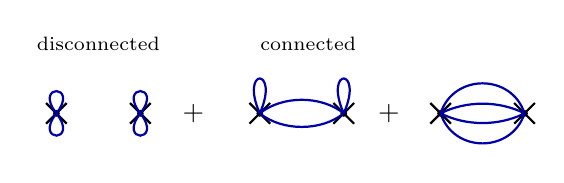
\begin{tikzpicture}[scale=0.82]
  \node at (-0.25,1.08) {\scriptsize disconnected};
  \foreach \x in {-0.9,0.4} {
    \fill (\x,0) circle (1.5pt);
    \draw[thick] (\x-0.16,-0.16) -- (\x+0.16,0.16);
    \draw[thick] (\x-0.16,0.16) -- (\x+0.16,-0.16);
    \draw[thick,blue!65!black]
      (\x,0) .. controls (\x-0.36,0.46) and (\x+0.36,0.46) .. (\x,0);
    \draw[thick,blue!65!black]
      (\x,0) .. controls (\x-0.36,-0.46) and (\x+0.36,-0.46) .. (\x,0);
  }
  \node at (1.22,0) {$+$};

  \node at (3.0,1.08) {\scriptsize connected};
  \foreach \x in {2.25,3.55} {
    \fill (\x,0) circle (1.5pt);
    \draw[thick] (\x-0.16,-0.16) -- (\x+0.16,0.16);
    \draw[thick] (\x-0.16,0.16) -- (\x+0.16,-0.16);
    \draw[thick,blue!65!black]
      (\x,0) .. controls (\x-0.32,0.72) and (\x+0.32,0.72) .. (\x,0);
  }
  \draw[thick,blue!65!black]
    (2.25,0) .. controls (2.6,0.28) and (3.2,0.28) .. (3.55,0);
  \draw[thick,blue!65!black]
    (2.25,0) .. controls (2.6,-0.28) and (3.2,-0.28) .. (3.55,0);
  \node at (4.25,0) {$+$};

  \foreach \x in {5.05,6.35} {
    \fill (\x,0) circle (1.5pt);
    \draw[thick] (\x-0.16,-0.16) -- (\x+0.16,0.16);
    \draw[thick] (\x-0.16,0.16) -- (\x+0.16,-0.16);
  }
  \draw[thick,blue!65!black]
    (5.05,0) .. controls (5.25,0.62) and (6.15,0.62) .. (6.35,0);
  \draw[thick,blue!65!black]
    (5.05,0) .. controls (5.25,-0.62) and (6.15,-0.62) .. (6.35,0);
  \draw[thick,blue!65!black]
    (5.05,0) .. controls (5.45,0.2) and (5.95,0.2) .. (6.35,0);
  \draw[thick,blue!65!black]
    (5.05,0) .. controls (5.45,-0.2) and (5.95,-0.2) .. (6.35,0);
\end{tikzpicture}
\end{center}

Let \(G^{(\ell)}\) be the sum of connected vacuum Wick contractions involving
\(\ell\) interaction vertices, including the coupling factors and integration
over the \(\ell\) vertex positions. If \(m_\ell\) is the number of connected
components of size \(\ell\), and if \(K\) is the total number of connected
components, then
\[
  \sum_{\ell\ge1}m_\ell=K,
  \qquad
  \sum_{\ell\ge1}\ell\,m_\ell=n.
\]
The number of ways to partition \(n\) labelled vertices into this pattern is
\[
  \frac{n!}{\prod_{\ell\ge1}(\ell!)^{m_\ell}m_\ell!}.
\]
For this fixed component pattern, the corresponding contribution to
\(Z_g/Z_0\) is therefore
\[
  \frac{1}{n!}\,
  \frac{n!}{\prod_{\ell\ge1}(\ell!)^{m_\ell}m_\ell!}
  \prod_{\ell\ge1}\bigl(G^{(\ell)}\bigr)^{m_\ell}
  =
  \prod_{\ell\ge1}
  \frac{1}{m_\ell!}
  \left(\frac{1}{\ell!}G^{(\ell)}\right)^{m_\ell}.
\]
Summing over all nonnegative integers \(m_\ell\) gives the linked-cluster
formula
\[
  \frac{Z_g}{Z_0}
  =
  \sum_{\{m_\ell\}}
  \prod_{\ell\ge1}
  \frac{1}{m_\ell!}
  \left(\frac{1}{\ell!}G^{(\ell)}\right)^{m_\ell}
  =
  \exp\left[
    \sum_{\ell\ge1}\frac{1}{\ell!}G^{(\ell)}
  \right].
\]
Equivalently, \(\log Z_g\) is the sum of connected vacuum diagrams.
The factor \(1/\ell!\) is often absorbed into the symmetry factor assigned to
the connected graph.

For example, the connected three-vertex topology with two propagators on each
edge has
\[
  N_\triangle=\binom{4}{2}^3(2!)^3=1728
\]
Wick-contraction assignments: at each vertex one chooses which two of the four
half-edges go to one neighboring vertex, and along each of the three double
edges one pairs the two half-edges.  Its contribution to
\(\frac{1}{3!}G^{(3)}\) is therefore
\begin{center}
\begin{tikzpicture}[baseline=-0.45ex,scale=0.78]
  \coordinate (a) at (0,0);
  \coordinate (b) at (1.55,0);
  \coordinate (c) at (0.78,1.08);
  \foreach \p in {a,b,c} {
    \fill (\p) circle (1.4pt);
    \draw[thick] ($(\p)+(-0.15,-0.15)$) -- ($(\p)+(0.15,0.15)$);
    \draw[thick] ($(\p)+(-0.15,0.15)$) -- ($(\p)+(0.15,-0.15)$);
  }
  \draw[thick,blue!65!black] (a) .. controls (0.45,0.23) and (1.1,0.23) .. (b);
  \draw[thick,blue!65!black] (a) .. controls (0.45,-0.23) and (1.1,-0.23) .. (b);
  \draw[thick,blue!65!black] (b) .. controls (1.18,0.47) and (1.08,0.72) .. (c);
  \draw[thick,blue!65!black] (b) .. controls (1.58,0.55) and (1.22,1.04) .. (c);
  \draw[thick,blue!65!black] (c) .. controls (0.48,0.72) and (0.37,0.47) .. (a);
  \draw[thick,blue!65!black] (c) .. controls (-0.02,1.04) and (-0.04,0.55) .. (a);
\end{tikzpicture}
\end{center}
\[
\begin{aligned}
  &\frac{1}{3!}
  \left(-\frac{g}{4!}\right)^3
  N_\triangle
  \int\dd\tau_1\,\dd\tau_2\,\dd\tau_3\,
  G_0(\tau_1,\tau_2)^2
  G_0(\tau_2,\tau_3)^2
  G_0(\tau_3,\tau_1)^2                                      \\
  &\hspace{4em}
  =
  -\frac{g^3}{48}\int\dd\tau_1\,\dd\tau_2\,\dd\tau_3\,
  G_0(\tau_1,\tau_2)^2
  G_0(\tau_2,\tau_3)^2
  G_0(\tau_3,\tau_1)^2,
\end{aligned}
\]
where the last equality uses the normalization \(4!\) in the interaction
vertex.  Translation invariance leaves one unrestricted
center-of-time integral, so every connected vacuum graph is proportional to
the total Euclidean time interval.

On a finite Euclidean interval of length \(T_{\mathrm{tot}}\), with endpoint
values \(q_i\) and \(q_f\), the path integral is the transition kernel
\[
  Z_g(T_{\mathrm{tot}};q_f,q_i)
  =
  \bra{q_f}\ee^{-T_{\mathrm{tot}}\widehat H}\ket{q_i}.
\]
For the anharmonic oscillator the spectrum is discrete and the ground state is
nondegenerate.  If the endpoint wavefunctions have nonzero overlap with the
ground state, the spectral theorem gives
\[
  Z_g(T_{\mathrm{tot}};q_f,q_i)
  =
  \psi_0(q_f)\overline{\psi_0(q_i)}
  \ee^{-E_0(g)T_{\mathrm{tot}}}
  +O(\ee^{-E_1(g)T_{\mathrm{tot}}}),
\]
and hence
\[
  E_0(g)
  =
  -\lim_{T_{\mathrm{tot}}\to\infty}
  \frac{1}{T_{\mathrm{tot}}}\log Z_g.
\]
The first correction is
\[
  \Delta E_0
  =
  \frac{g}{8}G_0(0)^2+O(g^2)
  =
  \frac{g}{32}+O(g^2),
\]
where the second equality uses \(\omega=1\); with general oscillator frequency
the same term is \(g(2\omega)^{-2}/8\).
This agrees with first-order Hamiltonian perturbation theory:
\[
  \bra{\psi_0}\frac{g}{4!}\widehat q^4\ket{\psi_0}
  =
  \frac{g}{4!}\,3\left(\frac12\right)^2
  =
  \frac{g}{32}.
\]

\section{Connected Two-Point Functions and Self-Energy}

The normalized Euclidean two-point function is
\[
  G(\tau)
  =
  \langle q(\tau)q(0)\rangle_g
  =
  \frac{1}{Z_g}
  \int[Dq]\,\ee^{-S_0[q]-S_{\mathrm{int}}[q]}\,q(\tau)q(0).
\]
Equivalently, at the regulated level,
\[
  G(\tau)
  =
  \frac{1}{Z_g}
  \left\langle
    q(\tau)q(0)
    \sum_{n=0}^{\infty}\frac{1}{n!}
    \left(-\frac{g}{4!}\int q(\tau')^4\,\dd\tau'\right)^n
  \right\rangle_0 .
\]
In the perturbative expansion, every Wick contraction splits uniquely into
the connected component containing the two external insertions and a product
of vacuum components. The sum of the vacuum components is \(Z_g\), and is
cancelled by the normalization. Thus \(G(\tau)\) is the sum of connected
two-point diagrams.

\begin{center}
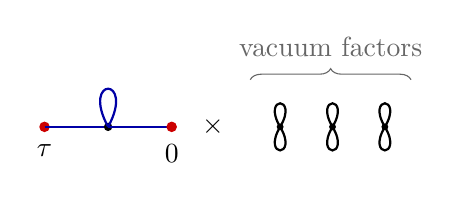
\begin{tikzpicture}[scale=0.95]
  \fill[red!80!black] (0,0) circle (2pt);
  \node[below=3pt] at (0,0) {$\tau$};
  \draw[thick,blue!65!black] (0,0) -- (0.85,0);
  \fill (0.85,0) circle (1.6pt);
  \draw[thick,blue!65!black]
    (0.85,0) .. controls (0.48,0.68) and (1.22,0.68) .. (0.85,0);
  \draw[thick,blue!65!black] (0.85,0) -- (1.7,0);
  \fill[red!80!black] (1.7,0) circle (2pt);
  \node[below=3pt] at (1.7,0) {$0$};
  \node at (2.25,0) {$\times$};
  \draw[decorate,decoration={brace,amplitude=4pt},gray!80!black]
    (2.75,0.63) -- node[midway,above=5pt] {vacuum factors} (4.9,0.63);
  \foreach \x in {3.15,3.85,4.55} {
    \draw[thick] (\x,0) .. controls (\x-0.25,0.42) and (\x+0.25,0.42) .. (\x,0);
    \draw[thick] (\x,0) .. controls (\x-0.25,-0.42) and (\x+0.25,-0.42) .. (\x,0);
    \fill (\x,0) circle (1.3pt);
  }
\end{tikzpicture}
\end{center}

Consequently the normalized correlator is represented by connected diagrams
with the two external insertions fixed at \(\tau\) and \(0\):
\begin{center}
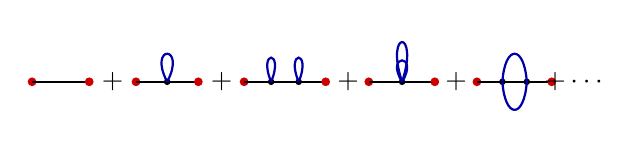
\begin{tikzpicture}[baseline=-0.5ex,scale=0.66]
  \fill[red!80!black] (0,0) circle (2.4pt);
  \draw[thick] (0,0) -- (1.1,0);
  \fill[red!80!black] (1.1,0) circle (2.4pt);
  \node at (1.55,0) {$+$};

  \fill[red!80!black] (2.0,0) circle (2.4pt);
  \draw[thick] (2.0,0) -- (3.2,0);
  \fill[red!80!black] (3.2,0) circle (2.4pt);
  \fill (2.6,0) circle (1.8pt);
  \draw[thick,blue!65!black] (2.6,0) .. controls (2.22,0.72) and (2.98,0.72) .. (2.6,0);
  \node at (3.65,0) {$+$};

  \fill[red!80!black] (4.08,0) circle (2.4pt);
  \draw[thick] (4.08,0) -- (5.65,0);
  \fill[red!80!black] (5.65,0) circle (2.4pt);
  \foreach \x in {4.6,5.13} {
    \fill (\x,0) circle (1.8pt);
    \draw[thick,blue!65!black] (\x,0) .. controls (\x-0.26,0.62) and (\x+0.26,0.62) .. (\x,0);
  }
  \node at (6.08,0) {$+$};

  \fill[red!80!black] (6.48,0) circle (2.4pt);
  \draw[thick] (6.48,0) -- (7.75,0);
  \fill[red!80!black] (7.75,0) circle (2.4pt);
  \fill (7.12,0) circle (1.8pt);
  \draw[thick,blue!65!black] (7.12,0) .. controls (6.78,0.55) and (7.46,0.55) .. (7.12,0);
  \draw[thick,blue!65!black] (7.12,0) .. controls (6.78,1.02) and (7.46,1.02) .. (7.12,0);
  \node at (8.16,0) {$+$};

  \fill[red!80!black] (8.56,0) circle (2.4pt);
  \draw[thick] (8.56,0) -- (10.0,0);
  \fill[red!80!black] (10.0,0) circle (2.4pt);
  \foreach \x in {9.05,9.52} {\fill (\x,0) circle (1.8pt);}
  \draw[thick,blue!65!black] (9.05,0) .. controls (9.1,0.72) and (9.47,0.72) .. (9.52,0);
  \draw[thick,blue!65!black] (9.05,0) .. controls (9.1,-0.72) and (9.47,-0.72) .. (9.52,0);
  \node at (10.42,0) {$+\cdots$};
\end{tikzpicture}
\end{center}
The same path integral, with the same Euclidean ordering convention, computes
\(\bra0\widehat q_E(0)\widehat q_E(\tau)\ket0\) when \(\tau<0\). Thus
\[
  G(\tau)
  =
  \begin{cases}
    \bra0\widehat q_E(\tau)\widehat q_E(0)\ket0, & \tau>0,\\
    \bra0\widehat q_E(0)\widehat q_E(\tau)\ket0, & \tau<0.
  \end{cases}
\]

At zeroth order,
\[
  G_0(\tau)=\frac12\ee^{-|\tau|}
  =
  \int_{-\infty}^{\infty}\frac{\dd k}{2\pi}\,
  \frac{\ee^{\ii k\tau}}{k^2+1}.
\]
At order \(g\), the connected tadpole correction is
\[
  -\frac{g}{2}
  \int \dd\tau'\,
  G_0(\tau-\tau')G_0(\tau')G_0(0).
\]
In momentum space this is
\[
\begin{aligned}
  &-\frac{g}{2}\int\dd\tau'\,
  \int\frac{\dd k}{2\pi}\frac{\dd k'}{2\pi}
       \frac{\dd k''}{2\pi}\,
  \widetilde G_0(k)\widetilde G_0(k')\widetilde G_0(k'')\,
  \ee^{\ii k(\tau-\tau')+\ii k'\tau'}                         \\
  &\hspace{4.5em}
  =
  -\frac{g}{2}
  \left(\int\frac{\dd k''}{2\pi}\,\widetilde G_0(k'')\right)
  \int\frac{\dd k}{2\pi}\,
  \frac{\ee^{\ii k\tau}}{(k^2+1)^2}.
\end{aligned}
\]
Since \(\int\dd k''\,\widetilde G_0(k'')/(2\pi)=G_0(0)=1/2\), this becomes
\[
  -\frac{g}{4}
  \int_{-\infty}^{\infty}\frac{\dd k}{2\pi}\,
  \frac{\ee^{\ii k\tau}}{(k^2+1)^2}.
\]

At second order the connected two-point graphs include
\begin{center}
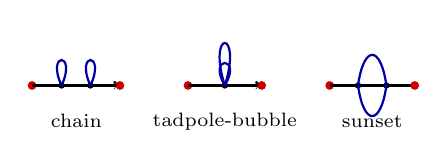
\begin{tikzpicture}[baseline=-0.5ex,scale=0.72]
  \fill[red!80!black] (0,0) circle (2.2pt);
  \draw[thick] (0,0) -- (1.55,0);
  \fill[red!80!black] (1.55,0) circle (2.2pt);
  \foreach \x in {0.52,1.03} {
    \fill (\x,0) circle (1.6pt);
    \draw[thick,blue!65!black] (\x,0) .. controls (\x-0.28,0.6) and (\x+0.28,0.6) .. (\x,0);
  }
  \node[font=\scriptsize] at (0.78,-0.63) {chain};
  \node at (1.95,0) {$,\qquad$};

  \fill[red!80!black] (2.75,0) circle (2.2pt);
  \draw[thick] (2.75,0) -- (4.05,0);
  \fill[red!80!black] (4.05,0) circle (2.2pt);
  \fill (3.4,0) circle (1.6pt);
  \draw[thick,blue!65!black] (3.4,0) .. controls (3.08,0.53) and (3.72,0.53) .. (3.4,0);
  \draw[thick,blue!65!black] (3.4,0) .. controls (3.08,1.0) and (3.72,1.0) .. (3.4,0);
  \node[font=\scriptsize] at (3.4,-0.63) {tadpole-bubble};
  \node at (4.45,0) {$,\qquad$};

  \fill[red!80!black] (5.25,0) circle (2.2pt);
  \draw[thick] (5.25,0) -- (6.75,0);
  \fill[red!80!black] (6.75,0) circle (2.2pt);
  \foreach \x in {5.75,6.25} {\fill (\x,0) circle (1.6pt);}
  \draw[thick,blue!65!black] (5.75,0) .. controls (5.85,0.72) and (6.15,0.72) .. (6.25,0);
  \draw[thick,blue!65!black] (5.75,0) .. controls (5.85,-0.72) and (6.15,-0.72) .. (6.25,0);
  \node[font=\scriptsize] at (6.0,-0.63) {sunset};
\end{tikzpicture}
\end{center}
The first diagram is a chain of two one-loop insertions; the other two are the
second-order amputated insertions that enter the self-energy below.

A connected two-point diagram is one-particle-irreducible, abbreviated
\(1\mathrm{PI}\), when it remains connected after cutting any one internal
propagator. In this chapter the term is graph-theoretic and refers to
Euclidean Green-function diagrams. Let \(\Sigma(k)\) be the sum of amputated
\(1\mathrm{PI}\) two-point insertions in momentum space. Then the full
two-point function is the geometric series
\[
  \widetilde G(k)
  =
  \widetilde G_0(k)
  \sum_{r=0}^{\infty}
  \bigl(\widetilde G_0(k)\Sigma(k)\bigr)^r
  =
  \frac{1}{k^2+1-\Sigma(k)},
  \qquad
  \widetilde G_0(k)=\frac{1}{k^2+1}.
\]

\begin{center}
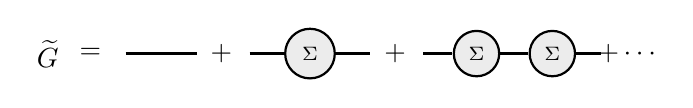
\begin{tikzpicture}[scale=0.9]
  \node at (-0.55,0) {$\widetilde G$};
  \node at (0.05,0) {$=$};
  \draw[thick] (0.55,0) -- (1.55,0);
  \node at (1.9,0) {$+$};
  \draw[thick] (2.3,0) -- (2.8,0);
  \draw[thick,fill=gray!15] (3.15,0) circle (0.35);
  \node at (3.15,0) {\scriptsize \(\Sigma\)};
  \draw[thick] (3.5,0) -- (4.0,0);
  \node at (4.35,0) {$+$};
  \draw[thick] (4.75,0) -- (5.15,0);
  \draw[thick,fill=gray!15] (5.5,0) circle (0.32);
  \node at (5.5,0) {\scriptsize \(\Sigma\)};
  \draw[thick] (5.82,0) -- (6.22,0);
  \draw[thick,fill=gray!15] (6.57,0) circle (0.32);
  \node at (6.57,0) {\scriptsize \(\Sigma\)};
  \draw[thick] (6.89,0) -- (7.25,0);
  \node at (7.62,0) {$+\cdots$};
\end{tikzpicture}
\end{center}

For the anharmonic oscillator, the two non-chain order-\(g^2\) contributions
are as follows.  The perturbative coefficient before Wick contraction is
\(g^2/(2(4!)^2)\).  For the tadpole-bubble topology, both external fields are
contracted to one interaction vertex, two lines connect the two vertices, and
the remaining two fields at the second vertex contract with each other.  The
number of such contractions is
\[
  2\cdot (4\cdot3)\cdot\binom42\,2! = 288,
\]
so the net symmetry factor is \(288/[2(4!)^2]=1/4\).  With
\[
  G_0(0)
  =
  \int_{-\infty}^{\infty}\frac{\dd p}{2\pi}\,\widetilde G_0(p)
  =
  \frac12,
  \qquad
  \int_{-\infty}^{\infty}\frac{\dd p}{2\pi}\,\widetilde G_0(p)^2
  =
  \frac14,
\]
this topology contributes
\[
  \Sigma_{\mathrm{tb}}^{(2)}(k)
  =
  \frac{g^2}{4}\,G_0(0)
  \int_{-\infty}^{\infty}\frac{\dd p}{2\pi}\,\widetilde G_0(p)^2
  =
  \frac{g^2}{32}
  =
  \frac{g^2}{8}\,\frac14 .
\]
For the sunset topology, the two external fields attach to different vertices
and the remaining three legs at one vertex are paired with the remaining three
legs at the other.  The contraction count is
\[
  2\cdot4\cdot4\cdot3! = 192,
\]
so the symmetry factor is \(192/[2(4!)^2]=1/6\).  Its momentum integral is the
three-fold convolution
\[
\begin{aligned}
  I_{\mathrm{sun}}(k)
  &=
  \int\frac{\dd p}{2\pi}\frac{\dd q}{2\pi}\,
  \widetilde G_0(p)\widetilde G_0(q)\widetilde G_0(k-p-q)  \\
  &=
  \int_{-\infty}^{\infty}\dd\tau\,\ee^{-\ii k\tau}G_0(\tau)^3
  =
  \frac18
  \int_{-\infty}^{\infty}\dd\tau\,\ee^{-\ii k\tau}\ee^{-3|\tau|}
  =
  \frac{3}{4}\,\frac{1}{k^2+9}.
\end{aligned}
\]
Thus
\[
  \Sigma_{\mathrm{sun}}^{(2)}(k)
  =
  \frac{g^2}{6}I_{\mathrm{sun}}(k)
  =
  \frac{g^2}{8}\,\frac{1}{k^2+9}.
\]
Combining the one-loop term with these two order-\(g^2\) contributions gives
\[
  \Sigma(k)
  =
  -\frac{g}{4}
  +
  \frac{g^2}{8}
  \left(
    \frac14+\frac{1}{k^2+9}
  \right)
  +O(g^3).
\]
The external free propagators are not part of \(\Sigma\); in this convention
the order-\(g\) term is the amputated tadpole, while the two displayed
order-\(g^2\) terms come from the two non-chain second-order topologies shown
above after their external legs are amputated.  The chain of two one-loop
insertions is instead produced by the geometric series in
\(\widetilde G_0(k)\Sigma(k)\).  Consequently
\[
  \widetilde G(k)
  =
  \frac{1}{
    k^2+1+\frac{g}{4}
    -\frac{g^2}{8}\left(\frac14+\frac{1}{k^2+9}\right)
    +O(g^3)
  }.
\]
The spectral expansion says that for \(\tau>0\),
\[
  G(\tau)
  =
  \sum_n
  \left|\bra n\widehat q\ket 0\right|^2
  \ee^{-(E_n-E_0)\tau}.
\]
The Fourier representation
\[
  G(\tau)
  =
  \int_{-\infty}^{\infty}\frac{\dd k}{2\pi}\,
  \widetilde G(k)\ee^{\ii k\tau}
\]
is evaluated for \(\tau>0\) by closing the contour in the upper half-plane,
where \(\ee^{\ii k\tau}\) decays on the large semicircle.
\begin{center}
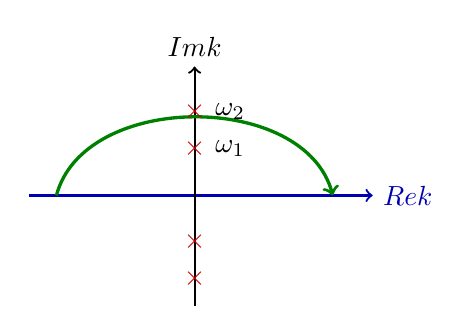
\begin{tikzpicture}[baseline=-0.45ex,scale=0.78]
  \draw[->,thick,blue!70!black] (-2.7,0) -- (2.9,0)
    node[right] {\(\operatorname{Re}k\)};
  \draw[->,thick] (0,-1.8) -- (0,2.1)
    node[above] {\(\operatorname{Im}k\)};
  \draw[very thick,green!50!black,->]
    (-2.25,0) .. controls (-1.8,1.7) and (1.8,1.7) .. (2.25,0);
  \foreach \y/\lab in {0.76/{\ii\omega_1},1.36/{\ii\omega_2}} {
    \node[red!80!black] at (0,\y) {\(\times\)};
    \node[right=4pt] at (0,\y) {\(\lab\)};
  }
  \foreach \y in {-0.75,-1.35} {
    \node[red!80!black] at (0,\y) {\(\times\)};
  }
\end{tikzpicture}
\end{center}
If
\(\widetilde G(k)\) has simple poles at \(k=\ii\omega_n\), then
\[
  G(\tau)
  =
  \ii\sum_n
  \operatorname*{Res}_{k=\ii\omega_n}\widetilde G(k)\,
  \ee^{-\omega_n\tau}.
\]
Thus the pole positions encode the energy gaps \(\omega_n=E_n-E_0\) in the
\(\hbar=1\) convention. The pole near \(k=\ii\) gives
\[
  E_1-E_0
  =
  1+\frac{g}{8}-\frac{g^2}{32}+O(g^3).
\]

\section{Derivative Interactions, Regulators, and Counterterms}

Consider the Lagrangian
\[
  L(q,\dot q)
  =
  \frac12\dot q^2-\frac12q^2-\frac{g}{8}q^2\dot q^2 .
\]
The canonical momentum is
\[
  p=\frac{\partial L}{\partial\dot q}
  =
  \dot q\left(1-\frac{g}{4}q^2\right),
\]
and the corresponding Hamiltonian function is
\[
  H(q,p)
  =
  \frac12\left(1-\frac{g}{4}q^2\right)^{-1}p^2
  +\frac12q^2.
\]
Already at the classical level this Hamiltonian shows the point that will
matter quantum mechanically: the product of the \(q\)-dependent coefficient
and \(p^2\) has no unique operator meaning until an ordering prescription, or
equivalently a regulated path-integral prescription, has been specified.

There is a useful classical check. Define a new coordinate \(y\), to first
order in \(g\), by
\[
  \frac{\dd y}{\dd q}
  =
  \left(1-\frac{g}{4}q^2\right)^{1/2},
  \qquad
  y=q-\frac{g}{24}q^3+O(g^2).
\]
Then \(q=y+\frac{g}{24}y^3+O(g^2)\), and the Lorentzian Lagrangian becomes
\[
  L
  =
  \frac12\dot y^2
  -
  \left(
    \frac12y^2+\frac{g}{24}y^4
  \right)
  +O(g^2).
\]
Thus the derivative-coupled oscillator is classically equivalent, through
order \(g\), to an ordinary anharmonic oscillator. The computation below keeps
the \(q\)-coordinate and shows where the quantum prescription enters.

The Euclidean Lagrangian is
\[
  L_E(q,q')
  =
  \frac12(q')^2+\frac12q^2-\frac{g}{8}q^2(q')^2 .
\]
Using
\[
  q^2(q')^2
  =
  \frac13\frac{\dd}{\dd\tau}(q^3q')
  -\frac13q^3q'',
\]
the interaction may also be represented, up to endpoint terms, by
\[
  \frac{g}{24}q^3q''.
\]

At first order in \(g\), the two-point function contains contractions in
which derivatives act on propagators at coincident points. A representative
term is
\[
  \frac{g}{4}\int\dd\tau'\,
  G_0(\tau-\tau')G_0(\tau')\,
  \left.
    \bigl[-\partial_{\tau'}^2G_0(\tau'-\tau'')\bigr]
  \right|_{\tau''=\tau'} .
\]
The derivative is taken with respect to one endpoint of the propagator before
the coincident-point limit \(\tau''\to\tau'\) is imposed.
In momentum space this contains
\[
  \int\frac{\dd k'}{2\pi}\frac{k'^2}{k'^2+1},
\]
which depends on the high-frequency definition of the path integral.
Other contractions in the same Wick expansion are finite or vanish by parity.
For example, with \(G_0(k)=1/(k^2+1)\), one obtains terms of the form
\[
  \frac{g}{4}
  \int\frac{\dd k}{2\pi}
    \frac{\ee^{\ii k\tau}k^2}{(k^2+1)^2}
  \int\frac{\dd k'}{2\pi}\frac{1}{k'^2+1},
\]
and
\[
  -\frac{g}{2}
  \int\frac{\dd k}{2\pi}
    \frac{\ee^{\ii k\tau}\ii k}{(k^2+1)^2}
  \int\frac{\dd k'}{2\pi}\frac{\ii k'}{k'^2+1}=0.
\]
The divergent term is local in the external momentum expansion; this is why a
local counterterm can absorb it.

\begin{figure}[H]
  \centering
  \resizebox{0.96\textwidth}{!}{%
  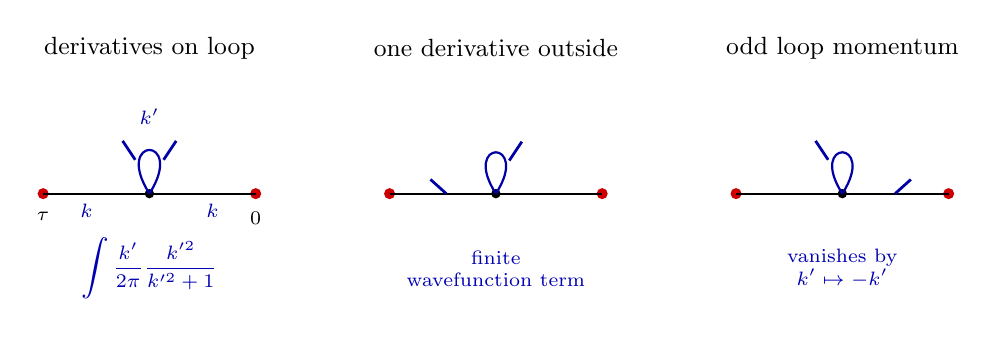
\begin{tikzpicture}[x=1cm,y=1cm,every node/.style={font=\scriptsize}]
    \begin{scope}
      \node[font=\small] at (1.35,1.85) {derivatives on loop};
      \coordinate (a) at (0,0);
      \coordinate (b) at (1.35,0);
      \coordinate (c) at (2.7,0);
      \fill[red!80!black] (a) circle (2pt);
      \node[below=3pt] at (a) {\(\tau\)};
      \fill[red!80!black] (c) circle (2pt);
      \node[below=3pt] at (c) {\(0\)};
      \fill (b) circle (1.7pt);
      \draw[thick] (a) -- (b) -- (c);
      \draw[thick,blue!65!black]
        (b) .. controls (0.88,0.74) and (1.82,0.74) .. (b);
      \draw[blue!65!black,line width=1pt] (1.17,0.43) -- (1.01,0.67);
      \draw[blue!65!black,line width=1pt] (1.53,0.43) -- (1.69,0.67);
      \node[blue!65!black] at (1.35,0.98) {\(k'\)};
      \node[blue!65!black] at (0.55,-0.22) {\(k\)};
      \node[blue!65!black] at (2.15,-0.22) {\(k\)};
      \node[align=center,blue!70!black] at (1.35,-0.95)
        {\(\displaystyle
        \int \frac{\dd k'}{2\pi}\frac{k'^2}{k'^2+1}\)};
    \end{scope}

    \begin{scope}[shift={(4.4,0)}]
      \node[font=\small] at (1.35,1.85) {one derivative outside};
      \coordinate (a) at (0,0);
      \coordinate (b) at (1.35,0);
      \coordinate (c) at (2.7,0);
      \fill[red!80!black] (a) circle (2pt);
      \fill[red!80!black] (c) circle (2pt);
      \fill (b) circle (1.7pt);
      \draw[thick] (a) -- (b) -- (c);
      \draw[thick,blue!65!black]
        (b) .. controls (0.90,0.70) and (1.80,0.70) .. (b);
      \draw[blue!65!black,line width=1pt] (1.52,0.42) -- (1.68,0.66);
      \draw[blue!65!black,line width=1pt] (0.72,0.0) -- (0.52,0.18);
      \node[align=center,blue!70!black] at (1.35,-0.95)
        {finite\\wavefunction term};
    \end{scope}

    \begin{scope}[shift={(8.8,0)}]
      \node[font=\small] at (1.35,1.85) {odd loop momentum};
      \coordinate (a) at (0,0);
      \coordinate (b) at (1.35,0);
      \coordinate (c) at (2.7,0);
      \fill[red!80!black] (a) circle (2pt);
      \fill[red!80!black] (c) circle (2pt);
      \fill (b) circle (1.7pt);
      \draw[thick] (a) -- (b) -- (c);
      \draw[thick,blue!65!black]
        (b) .. controls (0.90,0.70) and (1.80,0.70) .. (b);
      \draw[blue!65!black,line width=1pt] (1.17,0.43) -- (1.01,0.67);
      \draw[blue!65!black,line width=1pt] (2.02,0.0) -- (2.22,0.18);
      \node[align=center,blue!70!black] at (1.35,-0.95)
        {vanishes by\\\(k'\mapsto-k'\)};
    \end{scope}
  \end{tikzpicture}
  }
  \caption{Derivative interactions produce derivatives acting on Wick
  contractions.  When both derivatives act on the internal loop, the
  coincident-point contraction is sensitive to the high-frequency regulator.
  After cutoff regularization, the loop momentum \(k'\) in the first panel is
  restricted by \(|k'|<\Lambda\).  Other first-order contractions are finite or
  vanish by parity.}
  \label{fig:volume-i-derivative-interaction-contractions}
\end{figure}

The divergent expression is therefore not a value assigned by an already
defined continuum measure.  It is a signal that the formal product
\([Dq]=\prod_k \dd\widetilde q(k)\) must first be replaced by a regulated
finite-dimensional measure, and that the limiting prescription must be
specified together with local counterterms.

Define a frequency cutoff by
\[
  q(\tau)
  =
  \int_{|k|<\Lambda}\frac{\dd k}{2\pi}\,
  \widetilde q(k)\ee^{\ii k\tau},
  \qquad
  [Dq]_\Lambda=\prod_{|k|<\Lambda}\dd \widetilde q(k),
\]
with the real-field condition \(\widetilde q(k)^*=\widetilde q(-k)\). After
restoring \(\hbar\), the first-order self-energy has the form
\[
  \Sigma_\Lambda(k)
  =
  \frac{\hbar g}{4}
  \left(
    \frac{\Lambda}{\pi}
    +\frac{k^2}{2}
    -\frac12
    +O(\Lambda^{-1})
  \right)
  +O(\hbar^2g^2).
\]
A local Euclidean counterterm
\[
  \Delta L_E=C\,g\,\hbar\,\frac{q^2}{2}
\]
adds \(-Cg\hbar\) to \(\Sigma_\Lambda(k)\), so that
\[
  \Sigma_\Lambda(k)
  =
  \hbar g
  \left(
    \frac{k^2}{8}
    +\frac{\Lambda}{4\pi}
    -\frac18
    -C
    +O(\Lambda^{-1})
  \right)
  +O(g^2).
\]
Choosing
\[
  C=\frac{\Lambda}{4\pi}+C_{\mathrm{fin}}
\]
defines a finite limiting two-point function as \(\Lambda\to\infty\). The
finite constant \(C_{\mathrm{fin}}\) is part of the quantum definition of the
Hamiltonian represented by this regulated Lagrangian path integral.

The pole of the regulated two-point function,
\[
  \widetilde G_\Lambda(k)
  =
  \frac{\hbar}{k^2+1-\Sigma_\Lambda(k)},
\]
gives the first energy gap. Setting \(k=\ii\omega_1\) and expanding to first
order in \(g\) gives
\[
  \omega_1
  =
  1+\hbar g
  \left(
    -\frac{\Lambda}{8\pi}+\frac{C}{2}+\frac18
  \right)
  +O(g^2)
  =
  1+\hbar g
  \left(
    \frac{C_{\mathrm{fin}}}{2}+\frac18
  \right)
  +O(g^2).
\]
Thus the finite part of the local counterterm is not a removable notation
choice; it fixes which quantum Hamiltonian, within the ordering ambiguity of
the derivative-coupled classical expression, the path integral represents.
Once that quantum definition is fixed, the pole position is an ordinary
observable.

Fixing \(C_{\mathrm{fin}}\) requires physical input, for instance a
renormalization condition on the energy gap or an independently specified
operator ordering of the Hamiltonian.  In a relativistic field theory the
analogous finite local terms are constrained by Poincare covariance,
locality/microcausality, internal symmetries, and the chosen normalization
conditions on observables.

The structural statement carried forward to field theory is this: a path
integral with interactions is a regulated construction of Green functions,
and local counterterms are part of the data specifying the regulated
construction and its limiting prescription. The next chapter replaces the
single coordinate \(q(\tau)\) by fields \(\phi(x)\) and imposes relativistic
covariance and locality on the resulting Green functions.
